\chapter{Quality Assurance for relevance}
\label{ref:qa}

Especially in agile software development, quality assurance is incorporated into the standard software development workflow.
This often leads to resilient systems with high performance capabilities.
But for information retrieval systems, these are not always the most important goals.
As described in \autoref{ref:seanalysis}, a search engine should provide relevant results to the users.
Since the search engine itself is domain independent, 
it is not possible to ensure that a search engine provides relevant results for every domain.
Therefore the relevance criteria has to be covered in the \gls{glos:QA} process of the search service development.
The following sections will show, why the organization is an important influence on the quality of search results,
how the quality of search results can be measured in offline tests 
and what metrics are available to measure the relevance of search results experienced by the users.


\section{Relevance Aware Organizations}
\label{ref:qa:orga}
When implementing a new search service, software developers often
do not implement relevance metrics for their products,
since there is usually no requirement to do so.
The requirement to implement these metrics has to come from within an organization.
Only if all departments work together, relevant search results will be available for the user.
\par

In {\renewcommand{\mkbibbrackets}[1]{\textit{#1}}\cite{relevant_search_2016}} six levels of relevance-centered enterprises are described.
The following sections will outline each level and the characteristics of this level.
Every level has a corresponding feedback loop and every new level adds an additional feedback loop to the existing ones.
Each new feedback loop will have a shorter iteration (be smaller) than the previous one.
The feedback loop with the shortest iteration is reached when every request has it is own corresponding iteration.
This is called "\nameref{ref:qa:orga:l2r} " \cite[see][P. 276]{relevant_search_2016}.
Even if the inner feedback loops are looking good, an organization has to monitor all feedback loops 
to determine the current quality of the search results.
\begin{figure}[!ht]
	\centering
	\begin{tikzpicture}
								
		\def\oneexshift#1{\raisebox{1.0ex}}
		\draw[->,>=stealth',very thick,postaction={decorate,decoration={text along path,text align={center, left indent=1cm},text={|\scriptsize\oneexshift|Poor feedback/upset users/lost sales}}}] (150:150) arc[radius=3.0, start angle=260, end angle=-60];
		\draw[->,>=stealth',very thick,postaction={decorate,decoration={text along path,text align={center, left indent=0.8cm},text={|\scriptsize\oneexshift|Business and domain awareness}}}] (150:150) arc[radius=2.5, start angle=260, end angle=-65];
		\draw[->,>=stealth',very thick,postaction={decorate,decoration={text along path,text align={center, left indent=0.4cm},text={|\scriptsize\oneexshift|Content curation}}}] (150:150) arc[radius=2.0, start angle=260, end angle=-70];
		\draw[->,>=stealth',very thick,postaction={decorate,decoration={text along path,text align={center, left indent=0.2cm},text={|\scriptsize\oneexshift|Paired relevance tuning}}}] (150:150) arc[radius=1.5, start angle=260, end angle=-75];
		\draw[->,>=stealth',very thick,postaction={decorate,decoration={text along path,text align=center,text={|\scriptsize\oneexshift|Test-driven relevance}}}] (150:150) arc[radius=1.0, start angle=260, end angle=-80];
								
	\end{tikzpicture}
	\caption{Feedback loops of an relevance-centered enterprise}
	\label{fig:qa:orga:feedbackloops}
\end{figure}

\subsection{Flying relevance-blind}
\label{ref:qa:orga:blind}
The starting point of quality assurance for search service implementations is the relevance blindness.
Management, stakeholder and others do not have metrics to show them the quality of their search result relevance 
and therefore the resulting consequences stay unobserved \cite[see][P. 263]{relevant_search_2016}. 
Sometimes a whole search service gets implemented only to learn upon delivery, how disappointed the users are with the quality of the search results.
This situation is called "relevance-blind enterprise" and it can be very dangerous for the organization.
The corresponding feedback loop is the most outer one. Sales losses, customer complaints, etc. can be consequences of low quality search results.\\
Characteristics for this level are:
\begin{itemize}
	\item No relevance engineer, only back-end search engineers without an official relevance-tuning role.
	\item The search engine is used as a database and relevance scoring is mostly ignored.
	\item The frontend is overloaded with features like facet-filters etc, but ignores the ranking of the results.
\end{itemize}

\subsection{Business and domain awareness}
\label{ref:qa:orga:awarness}
This level is the first one having an enterprise internal feedback loop for the quality of search results.
The loop has to include different departments in an organization. Depending on the kind of application and organization,
the definition for "what users want" can be spread over many departments, such as marketing, sales, QA, legal,
consultants, management, etc. To figure out what the user wants, 
a relevance engineer has to break down the barriers between the departments and find the answers \cite[see][P. 265]{relevant_search_2016}.
This creates the first feedback loop, in which the departments give feedback on the quality of the search results.
Eventually, usability testing is performed in this stage to gather feedback from real users, who interact with the search service.\\
Characteristics for this level are:
\begin{itemize}
	\item Relevance engineer role exists.
	\item Internal feedback loop exists over multiple departments.
	\item \glspl{glos:domain:expert} consult the relevance engineers.
\end{itemize}

\subsection{Content curation}
\label{ref:qa:orga:contentcuration}
With a growing amount of internal feedback, it can easily happen, 
that the relevance engineers can not identify the "right answer" due to inconsistent answers from colleagues/departments.
The relevance engineers cannot focus on the technical improvements and are overwhelmed with the search feedback.
If this happens the "content curator" role should be created. 
The "content curator" is a role which is responsible to accept the feedback and determines the "right answer".
This means, that the content curator determines the order in which search results should be displayed for a given input.
The content curator has to balance the interests of all stake holders and forward the decisions to the relevance engineers,
which will focus on implementing the relevance decisions into the search service \cite[see][P. 268]{relevant_search_2016}.\par
In the agile methodology the content curator is similar to a product owner for the search service.
The communication between the content curator and the relevance engineers is crucial for this role to succeed.
Although the relevance engineers do not need to communicate with all departments anymore,
a certain level of direct communication is still needed to reduce the risk of miscommunication by the content curator.
This role creates a new feedback loop between the relevance engineers and the content curator,
which should be much faster, than the enterprise wide feedback loop.\\
Characteristics for this level are:
\begin{itemize}
	\item Content curator role exists.
	\item Direct and frequent communication between content curator and relevance engineers.
\end{itemize}

\subsection{Paired relevance tuning}
\label{ref:qa:orga:pairedrelevancetuning}
The next level of a relevance-centered enterprise consists of pairing between the content curator and the relevance engineers.
This method is similar to "pair programming", where two programmers work together to solve a programming problem.
In this case, the content curator and the relevance engineer solve the relevance problem by "pair tuning" \cite[see][P. 270-272]{relevant_search_2016}.
During "pair tuning" sessions, both are working at the same desk/computer to improve search relevance.
By using this method the next level of feedback loop is reached,
which consists of even faster iterations in the "pair tuning" sessions.
These iterations allow to identify issues fast and fix them with low effort.
The synergy effect of combining the expertise from two different specialists can be enormous.\\
Characteristics for this level are:
\begin{itemize}
	\item Pair tuning sessions with relevance engineers and the content curator.
	\item Relevance engineer and the content curator are sitting on the same desk.
\end{itemize}

\subsection{Test-driven relevance}
\label{ref:qa:orga:tdr}
Relevance tuning often results in situations comparable to a game of \gls{glos:whacamole}.
Every time one case is improved, the relevance of some other cases worsen.
It is nearly impossible to comprehend the whole effect of a change with all it is side effects.
Therefore another method is needed to not only improve the quality for some cases,
but to improve the overall quality of the search service.
\par
\gls{glos:unittesting} is a method from the traditional software development,
which allows a "divide and conquer" approach.
In this approach, the whole application is divided in units,
which are tested individually against some specified cases.
With enough test coverage, the software developer can be confident not to break existing functionality
when implementing new features, given all tests succeed.
\par
Test-driven relevance tuning is a technique which uses a similar method.
Test are created with a given query and some kind of result evaluation \cite[see][P. 272]{relevant_search_2016}.
These tests can come in two forms \cite[see][P. 273]{relevant_search_2016}:
\begin{enumerate}
	\item Judgement lists: A set of query/result combinations is created by the relevance engineer 
	      and the content curator and gets evaluated against the information retrieval system.
	\item Assertion-based testing: Some constraints are created for the expected results, 
	      e.g. when the user searches for "butter" the first result has to have the term "butter" in the title.
\end{enumerate}
Each of these two forms have their advantages and disadvantages.
Judgement lists help to see fine gradations in relevance quality, but also come with significant costs.
If the original dataset changes, the judgement lists have to be adapted. 
This leads to a constant change of the judgement lists, a task which can consume much effort and can not easily be outsourced since a basic domain expertise is needed.
Big organizations staff multiple departments of relevance testers to ensure the judgement lists are up to date\cite[see][section Evaluators]{google_search_2021}.\par
On the other hand, assertion-based testing is a good baseline to ensure a minimum quality for the search results exists.
Assertion-based tests are easy to maintain and come with a clear result.
Therefore they can be used for adhoc testing, since they either pass or fail.
Judgement lists do not have a binary result, usually some kind of score gets calculated to represent the quality of the results. 
Often it is useful to start with the creation of assertion tests and if all assertion tests are passed, judgement lists can be created and evaluated.
This method allows to document all the requirements before starting with the implementation of a search service.
\par
Another important effect is the measurability of relevance. 
Since the Judgement lists result in some kind of score,
the management can track the relevance improvements for each iteration.
With this metrics the management can gain a sense of control and evaluate investments in the relevance process.\\
Characteristics for this level are:
\begin{itemize}
	\item Automated tests are created in the form of assertion-based testing and judgement lists.
	\item Judgement lists are constantly maintained by the content curator and the relevance engineers.
\end{itemize}

\subsection{Learning to rank}
\label{ref:qa:orga:l2r}
Learning to rank is the final goal of the relevance improvement process.
It needs all other feedback loops to exist, before it can be implemented in a useful way.
Learning to rank allows the information retrieval system to improve itself automatically \cite[see][P. 276]{relevant_search_2016}.
E.g. a grocery e-commerce store sells fresh and frozen strawberries all over the year.
Usually the frozen strawberries are added to the cart, when a user searches for "strawberry".
But as soon as the local strawberry season starts, the fresh strawberries are sold more often.
This means that the relevance between the two products has to be switched.
In the winter months the frozen strawberries should be on the first position of the results,
but when the fresh strawberries are available, they should be on top of the result list.
Of course it is possible to handle this with manual intervention, 
in which the priorities of the products are switched as soon as the season starts.
However this can also be the opportunity for Learning to rank.
When the users start to buy the fresh strawberries, 
learning to rank should notice this and adapt the relevance of the fresh strawberries accordingly.
\par
It may make sense to use machine-learning models to generate automatic adaptions of the documents' relevance ratings.
The most known example of learning to rank is the page rank algorithm used by Google\cite[see][]{brin_page_1998}.
Another well known example is the usage of user interaction to determine the document relevance.
If the users interact more frequently with a document on the second position than with the document on the first position,
for a specific query, learning to rank can adapt the relevance of the second document to become the first one,
without the need of the interaction from a relevance engineer or the content curator.
To generate a domain specific learning to rank algorithm, it is important to combine the insights from all feedback loops
and extract the easily automated actions to a learning to rank algorithm.
It can be as easy as using the start and end date of the local strawberry season to put the fresh strawberries on the top of the search results.

\begin{figure}[!ht]
	\centering
	\begin{tikzpicture}
								
		\def\oneexshift#1{\raisebox{1.0ex}}
		\draw[->,>=stealth',very thick,postaction={decorate,decoration={text along path,text align={center, left indent=1cm},text={|\scriptsize\oneexshift|Poor feedback/upset users/lost sales}}}] (0,0) arc[radius=3.0, start angle=260, end angle=-60];
		\draw[->,>=stealth',very thick,postaction={decorate,decoration={text along path,text align={center, left indent=0.8cm},text={|\scriptsize\oneexshift|Business and domain awareness}}}] (0,0) arc[radius=2.5, start angle=260, end angle=-65];
		\draw[->,>=stealth',very thick,postaction={decorate,decoration={text along path,text align={center, left indent=0.4cm},text={|\scriptsize\oneexshift|Content curation}}}] (0,0) arc[radius=2.0, start angle=260, end angle=-70];
		\draw[->,>=stealth',very thick,postaction={decorate,decoration={text along path,text align={center, left indent=0.2cm},text={|\scriptsize\oneexshift|Paired relevance tuning}}}] (0,0) arc[radius=1.5, start angle=260, end angle=-75];
		\draw[->,>=stealth',very thick,postaction={decorate,decoration={text along path,text align=center,text={|\scriptsize\oneexshift|Test-driven relevance}}}] (0,0) arc[radius=1.0, start angle=260, end angle=-80];
								        
		\begin{scope}[shift={(0.15,1.0)}]
			\tstar{0.8}{1.05}{24}{0}{thick,fill=yellow}{0.5}{0.5};
			\node (a) at (0, 0.25) {\scriptsize Learning};
			\node (b) at (0, 0) {\scriptsize to};
			\node (c) at (0, -0.25) {\scriptsize Rank};
		\end{scope}
								                
	\end{tikzpicture}
	\caption{Learning to rank as the center of an relevance-centered enterprise}
	\label{fig:qa:orga:feedbackloopswithl2r}
\end{figure}

Since the knowledge of all other feedback loops is needed, learning to rank is the center of all feedback loops (See \autoref{fig:qa:orga:feedbackloopswithl2r}).
With the right expertise and data, it can be a extremely powerful tool to automatically improve relevance instantaneously.
Characteristics for this level are:
\begin{itemize}
	\item Automatic relevance-tuning by algorithms and machine learning
	\item User interaction is used as direct feedback in the automation
\end{itemize}

\section{Offline metrics}
\label{ref:qa:offlinemetrics}

As described, in \nameref{ref:qa:orga} some levels require metrics to improve the overall relevance.
Especially for \nameref{ref:qa:orga:tdr} metrics are needed, which can be evaluated against an implementation
without any user interaction. These metrics are called "Offline metrics".
%This type of metrics can be compared to unit tests in the software development.
Like assertions in the unit tests of traditional software development,
the relevance requirements are defined as a set of queries, with a list of expected results.
These lists were described in \nameref{ref:qa:orga:tdr} as "Judgment lists".
Unlike in software development, the goal is not to develop a search service,
which fulfills all requirements, but to create one which fulfills as many as possible, as good as possible.
This allows to develop the search service iteratively and improve it step by step with every iteration.
Therefore these metrics can not have a binary result like assertions in unit tests.
Usually, the results of these tests are a score, which is 100\% if all tests were fulfilled perfectly.
The calculation of this score is hard, since a search result can still be good, if the first two position of the results are swapped,
or if the second position is completely different than the expected second position.
In the following sections different methods are shown which can be used to calculate this score.
\par
All of the following metrics compare the expected results with the real results.
The term "Precision" is used to describe the percentage of documents in the result set that are relevant.
The term "Recall" is used to describe the percentage of relevant documents that are returned in the result set.
The following example shows how these two metrics are calculated for the query "apple".
This example simplifies documents by using only the title to represent the whole document.
In this example the expected result set for the term "apple" contains the documents: 
\begin{itemize}
	\item red apple
	\item green apple
	\item large apple
\end{itemize}
The result returned by the search service consists of the documents: 
\begin{itemize}
	\item red apple
	\item pomegranate
	\item large apple
	\item large tomato
	\item lemon
\end{itemize}
In the given example, the relevant documents are "red apple" and "large apple".
Therefore the precision is 40\%, because two of the five returned documents are relevant.
Also since two of three relevant documents were returned, the recall is 66.6\%.
\par
The goals for the relevance engineer are 100\% precision and 100\% recall, but these two goals are almost always mutually exclusive.
Usually, when the precision gets improved, the recall suffers and the other way around\cite[P. 77-78]{relevant_search_2016}.

\subsection{Precision at K (P@k)}
\label{ref:qa:offlinemetrics:patk}
This metric is based on the observation that users of a search service 
tend to use only the first $k$ results of a search result.
The metric measures the fraction of the $k$ results that are on average relevant for the given query.\cite[P. 416]{mcsherry_najork_2008}
The value of $k$ is also known as the "cut-off" value and it is assumed that $k\leq n$ is always true.
To calculate the metric, the result vector $V$ containing the results for the query is needed.
Also a function ($rel(v_i)$) has to be defined, which evaluates for a result ($v_i$) if it is relevant ($rel(v_i)=1$) or not ($rel(v_i)=0$).
\begin{equation}
	P@k(V) = \frac{\sum_{i=1}^{k} rel(v_i)}{k}
\end{equation}
This metric results in a score between zero and one, with one being a result containing only relevant documents 
and zero being a result without any relevant documents, for the first k results.
This metric does not give any information on the recall.

\subsection{Recall at K (R@k)}
\label{ref:qa:offlinemetrics:ratk}
This metrics gives information if all relevant documents are contained in the first $k$ search results.
Like in \nameref{ref:qa:offlinemetrics:patk} the result vector $V$ and the relevance function ($rel(v_i)$) have to be given.
This metric also needs the parameter $n$ which denotes the amount of documents available in the search result.\cite[P. 417]{mcsherry_najork_2008}
It can be assumed that $n$ is the number of all available documents and $V$ contains all available documents,
because an implementation would use a judgment list which would contain all relevant documents.
\begin{equation}
	R@k(V) = \frac{\sum_{i=1}^{k} rel(v_i)}{\sum_{i=1}^{n} rel(v_i)}
\end{equation}
This metrics results in a score between zero and one, with one being a result containing all relevant documents in the first $k$ search results
and zero being a result containing no relevant documents in the first $k$ search results.
This metric does give a little information on the precision of the search result, 
because $R@k=0 \implies P@k=0$ applies.

\subsection{Mean reciprocal rank}
\label{ref:qa:offlinemetrics:mrr}
Opposed to the first two metrics, the mean reciprocal rank does not rate the quality of a single query,
but the quality of a set of queries.
The set of queries is given as $Q$ and a single element of $Q$ is given as $q$.
For each query the position of the topmost ranked document is given as $r_q$, beginning with zero.
Also a cutoff $k$ is used and the ideal ranking would result in $MRR=1$ \cite[P. 89]{chakrabarti_khanna_sawant_bhattacharyya_2008}.
\begin{equation}
	MRR = \frac{1}{| Q |}\sum_{q \in Q}
	\begin{cases}
		1/(1+r_q) & r_q < k    \\
		0         & r_q \geq k 
	\end{cases}
\end{equation}
The resulting score is between zero and one, with one being the ideal score.
This metric is best suited for question-answer situations, where only one answer is correct.
A good example is a Google search for a domain name. The only relevant result is the website served on the given domain.

\subsection{Discounted cumulative gain (DCG)}
\label{ref:qa:offlinemetrics:dcg}
In \nameref{ref:qa:offlinemetrics:patk} and \nameref{ref:qa:offlinemetrics:ratk} documents are rewarded if they appear on the top of the search results.
The approach of discounted cumulative gain allows to punish relevant documents which appear at the end of the search results.
Therefore this metric supports "Graded Relevance"\cite[P. 1]{chapelle_metlzer_zhang_grinspan_2009}.
For this metric a gain function $G(x)$ needs to be defined, where $x$ is the relevance.
The gain function should return 0 if the document is not relevant and a positive rational number if the document is relevant.
For the parameter $x$ applies $x \in \{0,1\}$. One definition which is often used for the gain function is $G(rel_i) = 2^{rel_i} - 1$.
This metrics also needs a discount function $D(i)$ to be defined, where $i$ is the position of the current document in the search results.
The discount function is often implemented as $D(i) = \frac{1}{log_2(i+1)}$, with $i \in [1;\infty[$.
	
The given discount function punishes the results exponentially for each position further down in the search results.
Also a cutoff $k$ is used for this metric\cite[P. 420]{mcsherry_najork_2008}.
		
\begin{equation}
	DCG@k(V) = \sum_{i=1}^{k} G(rel(v_i))*D(i)
\end{equation}
This metric allows to refine the score for precision, but recall is neglected for results outside of $k$.
Also results with irrelevant documents at the end of the result set are scored equally to result sets with less, but only relevant documents.
It can make sense to use this metric in e-commerce search services, 
since it is acceptable to have the most relevant result on the second position in the result set.
The score has to get worse drastically when a relevant document is further down on the result set.
Another use case is the search for web documents, where the same scope for the relevance rating of the documents is given.\cite[P. 1]{chapelle_metlzer_zhang_grinspan_2009}
		
\subsection{Expected reciprocal rank (ERR)}
\label{ref:qa:offlinemetrics:err}
Even though \nameref{ref:qa:offlinemetrics:dcg} is a good metric for relevance judgement,
it neglects the user interaction with the documents.
The interaction of the user with a document in a result set does not only depend on the position of the document.
Often users which are not satisfied with the documents above $i$ are likely to explore the documents on $i$ and below.
A good example on how DCG fails to consider this is the following case:
Two lists are given, one list having 20 good results and another one with the perfect result on top followed by 19 irrelevant results.
DCG would consider the first list better, even without the perfect result.
But in reality a user would likely have the second result set, since it contains the perfect result on top.
\par
It is shown that on average DCG overestimates the relevance of a document on a later position for a user\cite[P. 3]{chapelle_metlzer_zhang_grinspan_2009}.
This can be explained by the click-through rates. If a user finds a satisfying result, all other results behind that result are irrelevant.
Therefore, a search result is only as relevant as the documents before the satisfying documents. 
All other documents should have a little to no effect on the relevance score.
Therefore, relevance for a given user should be modeled as the probability for a document that a random user is satisfied by it.
In ERR this probability is defined with $g_i$ being the grade of the $i$-th document as:
\begin{equation}
	R_i := \mathcal{R}(g_i)
\end{equation}
Here $\mathcal{R}(g)$ assign's from the grade to the probability of relevance.
When a document is not relevant $g_i = 0 \implies \mathcal{R}(g_i) = 0$ applies. 
On the basis of the gain function of DCG $\mathcal{R}(g)$ can be chosen as:
\begin{equation}
	\mathcal{R}(g) := \frac{2^g-1}{2^{g_max}}, \qquad g \in \{0,...,g_max\}
\end{equation}
For a five point scale of $g$ this means that $\mathcal{R}(4)$ (representing the probability of relevance) is near 1.
With $\mathcal{R}(g)$ defined, the resulting metric is defined as:
\begin{equation}
	ERR = \sum_{r=1}^{n} 1/r \prod_{i=1}^{r-1} (1-R_i)R_r
\end{equation}
This allows to calculate a score between zero and one, with one representing the perfect result set\cite[P. 4]{chapelle_metlzer_zhang_grinspan_2009}.
Usually, the judgment lists used for this metric are influenced by the click-through rates measured.
The calculated score should be a good model for the real document relevance to a user,
especially when online metrics (e.g. click-through rates) are used to influence the judgment lists.
This metric is useful to create and improve existing Information Retrieval Systems for e-commerce, web documents, etc.,
since it is an improvement over DCG and also correlates strongly with the click-through rate of real users.
\pagebreak		

\section{Online metrics}
\label{ref:qa:onlinemetrics}
Even the best \nameref{ref:qa:offlinemetrics} are just a model of the reality and can only be as good as the given judgment lists.
Therefore another type of metrics has to be used to determine if the given assumptions of the judgment lists are depicted in reality.
Online metrics are created by real users who interact with the Information Retrieval Systems.
These metrics can be captured as events. Usually at least two types of events are used, which are linked to a single so called "Search Fact".
The first event is the "search query" event, which reflects a users search query with all parameters.
The second event is the "search result interaction" event, which reflects an interaction with a search result document.
The resulting search fact has to have at least the "search query" event associated and if a user interaction happened,
also the "search result interaction" is linked to the search fact.
Therefore, the search fact contains the aggregated information which documents were interacted with for a specific query\cite{shopify_engineering_2021}.
A minimal example of the data structures used to gather online metrics is shown in \autoref{fig:qa:onlinemetrics:events}.
		
\begin{figure}[!ht]
	\centering
	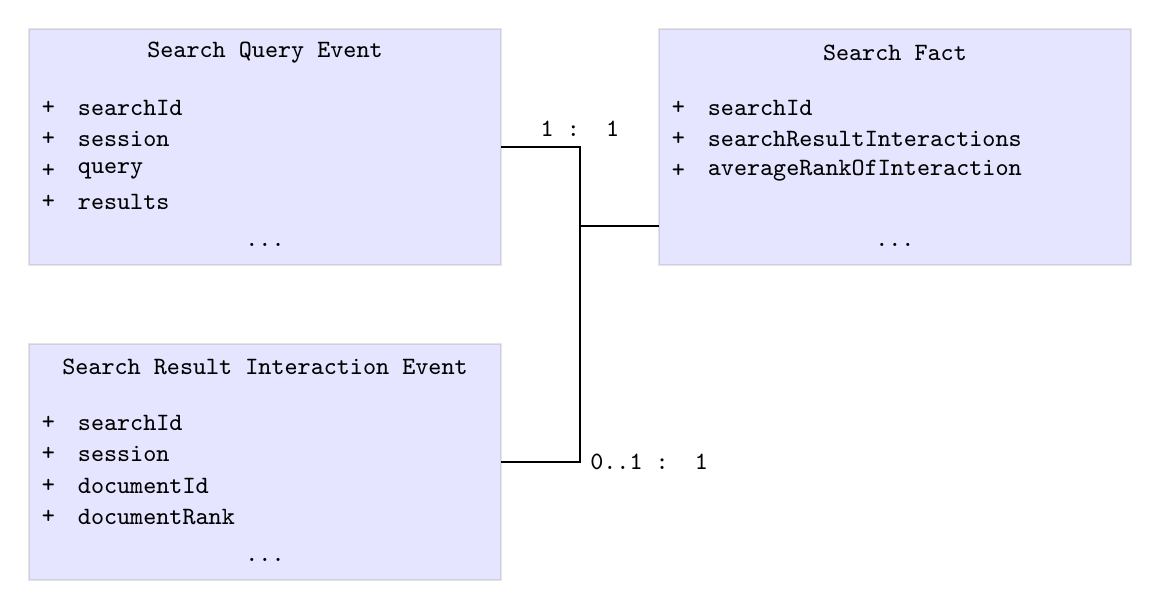
\begin{tikzpicture}[font=\small\ttfamily]
		% Search Query Event
		\draw[thick, fill=blue, opacity=0.1] (0, 4) rectangle ++(6,3);
		\node at (3,6.7) {\textbf{Search Query Event}};
		\path (0.25,6.0) node{+} ++(0.25,0) node[right]{searchId};
		\path (0.25,5.6) node{+} ++(0.25,0) node[right]{session};
		\path (0.25,5.2) node{+} ++(0.25,0) node[right]{query};
		\path (0.25,4.8) node{+} ++(0.25,0) node[right]{results};
		\node at (3,4.25) {...};
		
		% Search Result Interaction Event
		\draw[thick, fill=blue, opacity=0.1] (0, 0) rectangle ++(6,3);
		\node at (3,2.7) {\textbf{Search Result Interaction Event}};
		\path (0.25,2.0) node{+} ++(0.25,0) node[right]{searchId};
		\path (0.25,1.6) node{+} ++(0.25,0) node[right]{session};
		\path (0.25,1.2) node{+} ++(0.25,0) node[right]{documentId};
		\path (0.25,0.8) node{+} ++(0.25,0) node[right]{documentRank};
		\node at (3,0.25) {...};

		% Search Fact
		\draw[thick, fill=blue, opacity=0.1] (8, 4) rectangle ++(6,3);
		\node at (11,6.7) {\textbf{Search Fact}};
		\path (8.25,6.0) node{+} ++(0.25,0) node[right]{searchId};
		\path (8.25,5.6) node{+} ++(0.25,0) node[right]{searchResultInteractions};
		\path (8.25,5.2) node{+} ++(0.25,0) node[right]{averageRankOfInteraction};
		\node at (11,4.25) {...};

		% Connections
		\draw[thick] (6,5.5) -- (7,5.5) node[above] {1 : 1} -- (7, 4.5) -- (8,4.5);
		\draw[thick] (6,1.5) -- (7,1.5) node[right] {0..1 : 1}  -- (7, 4.5) -- (8,4.5);
	\end{tikzpicture}
	\caption{Data model for Online Metric Events}
	\label{fig:qa:onlinemetrics:events}
\end{figure}
		
The data for online metrics is often collected from search logs.
This allows to determine how real search events perform.
The most commonly used strategy to evaluate different search service versions are A/B tests.
		
\subsection{A/B Testing}
A/B Testing is a strategy which allows to compare multiple versions of a component.
It is possible to have two, three (this is called an A/B/C Test) or even more versions, which are evaluated against each other.
Also it is important to have one version acting as a control group.
To determine which version is better, a metrics has to be defined and evaluated.
It is important to test both versions simultaneously, 
because different circumstances at different times can influence the metric and therefore the test.
When testing simultaneously both versions must have the same circumstances.
The setup of an A/B test requires to split the audience into multiple groups\cite{chopra_2010}.
\par
For search services A/B test groups should be set up in a way to represent every user category equally in both groups.
E.g. a grocery shop search should not split the groups by region, or have a significantly lager portion of user from one region than from another,
because the region can influence what people are searching for. 
In Germany there are multiple names for red cabbage, it is either "Rotkohl" (red cabbage) in northern Germany and "Blaukraut" (blue herb) in the south of Germany.
\par
Next to the metrics and the group split, the duration of an A/B test is very important.
Usually, the duration can be calculated by the "statistical confidence".
It is important to ensure, that the A/B test has enough "statistical confidence", but is not running too long. 
It can happen that users are annoyed if they are in the group which is performing worse and eventually will not use the service anymore. 
Some common questions, which should often be answered by an A/B test are:
\begin{itemize}
	\item How often did users interact with search results?
	\item How far did they have to scroll to find the best result for their needs?
	\item Did they give up using the search service to achieve their goal?
\end{itemize}
In the next sections metrics are listed which can help to answer these questions.
Every metric has to be calculated for every group.
In an information retrieval system exposed to the Internet, 
\glspl{glos:robot:bot} will stop the metrics from achieving perfect results,
since they either interact with every given result or none of the given results.
If possible searches produced by \glspl{glos:robot:bot} should never be part of an A/B test.
		
\subsection{Click-through rate (CTR)}
The Click-through rate calculates the portion of users who interacted with a search result.
It can be calculated by counting all search requests $n_s$ and all interactions $n_i$ with the search results.
It is assumed that for each search request only one interaction can be made.
Since users will usually only interact with relevant results, 
this metric allows to measure the overall relevance of search results for users.
When $n_s$ and $n_i$ is given, then the following definition of CTR applies:
\begin{equation}
	CTR := \frac{n_i}{n_s}, \qquad n_i \leq n_s, n_s \in [1;\infty[
\end{equation}
The calculated CTR metric will have a value between zero and one, where zero is the worst and one is the best score.

\subsection{Average rank (AR)}
Since users want to have the most relevant result on the first place in the search results, 
the average rank metric provides a method to calculate the position of the relevant result in the search results.
When the number of interactions is $n$ and the search result rank for each interaction $i$ is given as $r_i$
the following definition applies:
\begin{equation}
	AR := \frac{n}{\sum_{i=0}^n r_i}, \qquad r_i \geq 1, n \in [1;\infty[
\end{equation}
The calculated AR metric will have a value between zero and one, where zero is the worst and one is the best score.
In the optimal case $r_i=1,i\in[0,n]$ would apply.
		
\subsection{Abandonment (AB)}
If users do not find any relevant result, they will usually not interact with any of the given documents.
They will either try again with a different query or leave the service completely.
This behavior can be measured with the Abandonment (AB) metric.
When $n_s$ and $n_i$ is given, then the following definition of AB applies:
\begin{equation}
	AB := 1 - \frac{n_s - n_i}{n_s}, \qquad n_i \leq n_s, n_s \in [1;\infty[
\end{equation}
The calculated AB metric will have a value between zero and one, where zero is the worst and one is the best score.
		
\subsection{Deflection}
Another metric, which is hard to measure, is the deflection.
It is defined as the number of users which have not contacted the provider of a search service, 
because they are able to find the documents needed.
This metric is also an important part in the \nameref{ref:qa:orga:awarness} feedback loop.
It needs a lot of business insights to be defined correctly,
though should be defined in the domain context and measured by educated customer service staff,
which should have the goal to reduce the amount of contacts needed by the users.
\par
In the case of Shopify, they tried to increase the deflection by improving their search service.
But of course there are cases where a users needs to contact the customer service,
even if the provided search results are the most relevant information.
Therefore it is important to get feedback from the customer service,
how many users had problems, which could be solved without contacting the customer service
and how many of them tried to find relevant information with the existing search service.\cite{shopify_engineering_2021}
